La palabra metodología está compuesta por tres vocablos griegos, los cuales son: metá (``más allá''), odós (``camino'') y logos (``estudio''). Es por ello que al conjunto de medios que se pueden utilizar para llegar a un fin para luego determinar cuál es el más adecuado se le denomina metodología.

Las metodologías de desarrollo de software ayudan a estructurar, planificar y controlar el proceso de desarrollo de los sistemas de información, con el objetivo de resolver las siguientes preguntas:

\begin{itemize}
    \item ¿Quién debe hacerlo?
    \item ¿Qué debe hacer?
    \item ¿Cuándo debe hacerlo?
    \item ¿Cómo debe hacerlo?
\end{itemize}

Este marco de trabajo es un modo sistemático de realizar, gestionar y administrar un proyecto con la posibilidad de llevarlo al éxito. Cada metodología de desarrollo de software tiene ciertas actividades las cuales ayudan a idear, implementar y mantener el producto de software, el cual surge de alguna necesidad hasta cumplir con el objetivo por el cual fue creado. Por lo último mencionado, se propuso la necesidad de metodizar el desarrollo de software, para lo cual se han hecho muchos esfuerzos para mejorarlo con el tiempo. Todo comenzó por los modelos carentes de disciplina y estándares, luego evolucionó a modelos estructurados centrados en el control del proceso (denominados metodologías tradicionales) y por último se dio paso a modelos iterativos y flexibles (metodologías ágiles).

Existe una constante guerra para determinar qué tipo de metodología es mejor que la otra, pero surgen preguntas como: ¿existe una mejor que la otra? o ¿cuál de estas llevará al éxito? 

Respondiendo a las últimas preguntas mencionadas, no existe una metodología mejor que otra ya que su elección también depende del proyecto en el que se utilicen. En efecto, factores tales como recursos técnicos y humanos, tiempo de desarrollo, tipo de sistema, etc. pueden condicionar la elección o aplicación de una metodología específica. Además, no existe metodología que asegure el éxito ya que todas pueden fracasar, lo importante es saber abordar los problemas y decidir qué tipo de metodología ocupar. Cada metodología posee algo bueno y en algunos casos se pueden mezclar, pero depende de las características del proyecto.

\begin{figure}[h]
  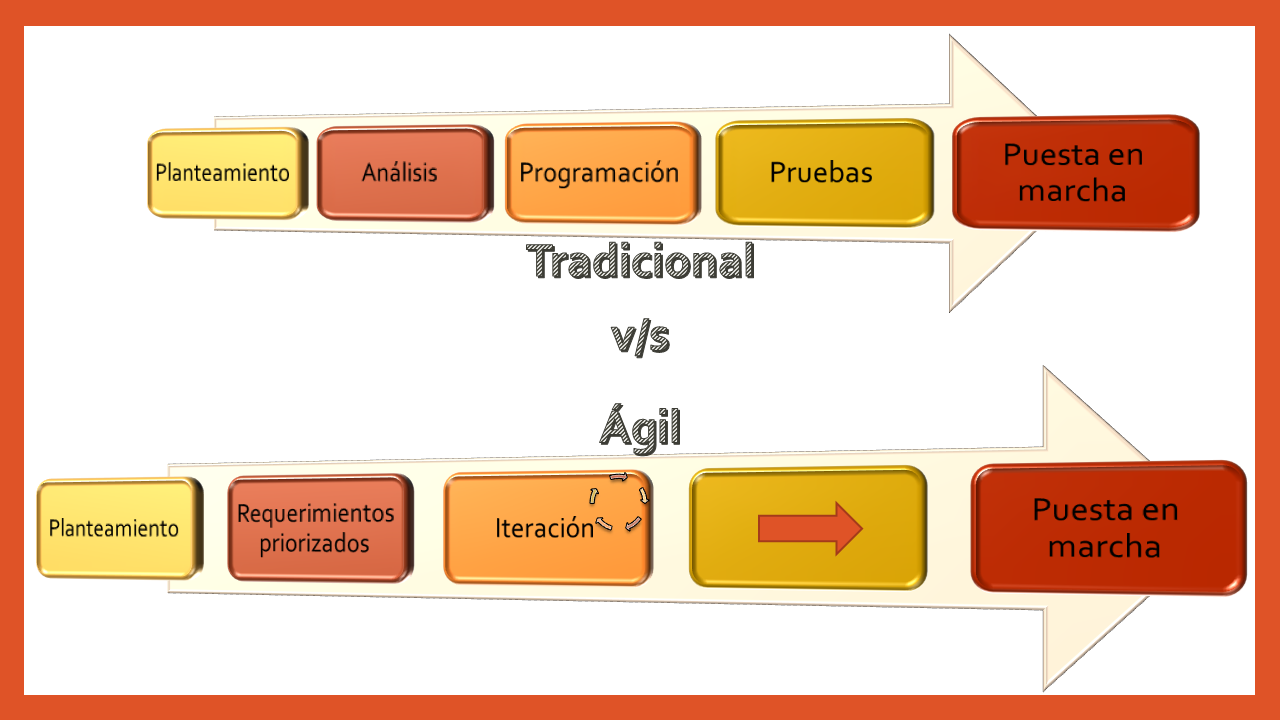
\includegraphics[width=\textwidth]{Imagenes/tradicional_vs_agil.png}
  \caption{\label{fig: dif_Metodologia} Metodología tradicional vs metodología ágil  ~\cite{17}.}
\end{figure}


\begin{table}[htb]
    
    \caption{\label{tab: tab_dif_Metodologia} Metodología Tradicional vs Metodología Ágil ~\cite{17}. }
    \footnotesize
    \begin{tabular}{| l || c | c |}
    
    \hline
      & \textbf{Tradicional} & \textbf{Ágil} \\
    
    \hline\hline
    
    \textbf{Enfoque} & Predictivo & Adaptativo\\ \hline

    \textbf{Éxito de medición}   & Conformación de planificar & Valor del negocio\\ \hline

    \textbf{Tamaño del proyecto} & Grande & Pequeño\\ \hline

    \textbf{Estilo de gestión} & Autocrático & Desentralizada \\ \hline

    \textbf{Perspectiva para el cambio} & Cambio y sostenibilidad & Cambio y adaptabilidad\\ \hline

    \textbf{Cultura} & Comandos de control & Liderazgo-Colaboración\\ \hline

    \textbf{Documentación} & Pesado & Bajo\\ \hline

    \textbf{Cliente} & Interactúa mediante reuniones & Parte del equipo\\ \hline

    \textbf{Énfasis} & Orientado a procesos & Orientado a personas\\ \hline
    
    \textbf{Ciclos} & Limitados & Muchos\\ \hline
    
    \textbf{Planificación por adelantado} & Exhaustivo & Mínimo\\ \hline
    
    \textbf{Retorno de la inversión} & Fin del proyecto & A principios del proyecto\\ \hline

    \textbf{Tamaño del equipo} & Grandes & Pequeños\\ \hline
    \end{tabular}  
\end{table}

En cuanto a la elección de la metodología que se utiliza, existen un sinfín de factores que diferencia entre una y otra, tal como se puede apreciar en la \textbf{Figura~\ref{fig: dif_Metodologia}}  y en el \textbf{Cuadro~\ref{tab: tab_dif_Metodologia}}. Es por ello que dada esta información y principalmente por los factores tales como Cliente, Tamaño del equipo, Ciclos, Perspectiva al cambio y Enfoque es que se optó por elegir la Metodología Ágil de la cual se da mayor énfasis en el siguiente ítem de este documento.